%% This is file `elsarticle-template-1-num.tex',
%%
%% Copyright 2009 Elsevier Ltd
%%
%% This file is part of the 'Elsarticle Bundle'.
%% ---------------------------------------------
%%
%% It may be distributed under the conditions of the LaTeX Project Public
%% License, either version 1.2 of this license or (at your option) any
%% later version.  The latest version of this license is in
%%    http://www.latex-project.org/lppl.txt
%% and version 1.2 or later is part of all distributions of LaTeX
%% version 1999/12/01 or later.
%%
%% Template article for Elsevier's document class `elsarticle'
%% with numbered style bibliographic references
%%
%% $Id: elsarticle-template-1-num.tex 149 2009-10-08 05:01:15Z rishi $
%% $URL: http://lenova.river-valley.com/svn/elsbst/trunk/elsarticle-template-1-num.tex $

%%%%%%%%%\documentclass[final,1p, times, twocolumn]{elsarticle}

%% Use the option review to obtain double line spacing
 \documentclass[preprint,review,12pt]{elsarticle}

%% Use the options 1p,twocolumn; 3p; 3p,twocolumn; 5p; or 5p,twocolumn
%% for a journal layout:
%% \documentclass[final,1p,times]{elsarticle}
%% \documentclass[final,1p,times,twocolumn]{elsarticle}
%% \documentclass[final,3p,times]{elsarticle}
%% \documentclass[final,3p,times,twocolumn]{elsarticle}
%% \documentclass[final,5p,times]{elsarticle}
%% \documentclass[final,5p,times,twocolumn]{elsarticle}

%% The graphicx package provides the includegraphics command.
\usepackage{graphicx}
%% The amssymb package provides various useful mathematical symbols
\usepackage{amssymb}
%% The amsthm package provides extended theorem environments
%% \usepackage{amsthm}

%% The lineno packages adds line numbers. Start line numbering with
%% \begin{linenumbers}, end it with \end{linenumbers}. Or switch it on
%% for the whole article with \linenumbers after \end{frontmatter}.
\usepackage{lineno}
\usepackage{siunitx}
%% natbib.sty is loaded by default. However, natbib options can be
%% provided with \biboptions{...} command. Following options are
%% valid:

\usepackage{caption}
\usepackage{subcaption}
\usepackage{hyperref}
\usepackage{float}
%%   round  -  round parentheses are used (default)
%%   square -  square brackets are used   [option]
%%   curly  -  curly braces are used      {option}
%%   angle  -  angle brackets are used    <option>
%%   semicolon  -  multiple citations separated by semi-colon
%%   colon  - same as semicolon, an earlier confusion
%%   comma  -  separated by comma
%%   numbers-  selects numerical citations
%%   super  -  numerical citations as superscripts
%%   sort   -  sorts multiple citations according to order in ref. list
%%   sort&compress   -  like sort, but also compresses numerical citations
%%   compress - compresses without sorting
%%
%% \biboptions{comma,round}

% \biboptions{}

%% \usepackage{authblk}
%% authors package


\graphicspath{{../figures/}}
\journal{Nuclear Instruments and Methods in Physics Research}

\begin{document}

\begin{frontmatter}

%% Title, authors and addresses

\title{MiniPIX Cosmic Ray Tracking and Radiation Dosimetry During SORA Stratospheric Balloon Flights}
%% title is a work in progress...

%% use the tnoteref command within \title for footnotes;
%% use the tnotetext command for the associated footnote;
%% use the fnref command within \author or \address for footnotes;
%% use the fntext command for the associated footnote;
%% use the corref command within \author for corresponding author footnotes;
%% use the cortext command for the associated footnote;
%% use the ead command for the email address,
%% and the form \ead[url] for the home page:
%%
%% \title{Title\tnoteref{label1}}
%% \tnotetext[label1]{}

% To avoid any authorship arguments I would suggest we order authors in alphabetical order by last name. Just a thought.
\author{S.~A.~Garcia~Morelos\fnref{label6}}%corresponding author
\author{A.~Walker\fnref{label2}}%corresponding author
\author{R.~B.~Masek\fnref{label4}}
\author{S.~Oliver\fnref{label5}}
\author{F.~Brooks\fnref{label7}}
\author{K.~D.~Portillo\fnref{label3}}
\author{J.~Patel\fnref{label11}}
\author{D.~Pattison\fnref{label17}}
\author{A.~L.~Renshaw\fnref{label10}}
%% \ead{email address}
%% \ead[url]{home page}
%% \fntext[label2]{}
%% \cortext[cor1]{}
%% \address{Address\fnref{label3}}
%% \fntext[label3]{}


%% use optional labels to link authors explicitly to addresses:
%% \author[label1,label2]{<author name>}
%% \address[label2]{<address>}
%% \address[label3]{<address>}

\address[label2,label3,label4,label5,label6,label7,label8,label9,label10,label11]{Department of Physics, University of Houston, Houston, TX 77204, USA}
\address[label17]{Department of Biology and Microbiology, University of Houston, Houston, TX 77204, USA}
%\address[label3]{Department of Physics, University of Houston, Houston, TX 77204, USA}
%\address[label4]{Department of Physics, University of Houston, Houston, TX 77204, USA}
%\address[label5]{Department of Physics, University of Houston, Houston, TX 77204, USA}
%\address[label6]{Department of Physics, University of Houston, Houston, TX 77204, USA}
%\address[label7]{Department of Physics, University of Houston, Houston, TX 77204, USA}
%\address[label8]{Department of Physics, University of Houston, Houston, TX 77204, USA}
%\address[label9]{Department of Physics, University of Houston, Houston, TX 77204, USA}
%\address[label10]{Department of Physics, University of Houston, Houston, TX 77204, USA}
%\address[label11]{Department of Physics, University of Houston, Houston, TX 77204, USA}


%% \author{John Smith}
%% \address{California, United States}
%% \newcommand{\Houston}{Department of Physics, University of Houston, Houston, TX 77204, USA}
%--- Add other authors in the order they should appear
%Abstract
%A concise and factual abstract is required. The abstract should state briefly the purpose of the research, the principal results and major conclusions. An abstract is often presented separately from the article, so it must be able to stand alone. For this reason, References should be avoided, but if essential, then cite the author(s) and year(s). Also, non-standard or uncommon abbreviations should be avoided, but if essential they must be defined at their first mention in the abstract itself.

\begin{abstract}

The latest results from the two radiation experiments onboard the Stratospheric Organisms and Radiation Analyzer (     ), high altitude balloon flights are presented.  The SORA payload included a semiconductor pixel detector, the MiniPIX, for cosmic ray studies and imaging in the stratosphere at altitudes of 30 to 40 kilometers.  The MiniPIX was interfaced with a low-powered  computer, a Raspberry Pi 3. The MiniPIX was set to TOT (time over threshold mode) and monitored cosmic radiation for a total flight time of 19.5 hours on two separate flights.  The results from the SORA flights were evaluated for providing a basis for future low cost cosmic ray tracking platforms on high altitude balloons and satellites.
%may require more citations for SORA, MiniPIX and Raspberry Pi

\end{abstract}

%Required Structure: https://www.elsevier.com/journals/nuclear-instruments-and-methods-in-physics-research-section-a-accelerators-spectrometers-detectors-and-associated-equipment/0168-9002/guide-for-authors

%optional: Highlights
%Highlights are a short collection of bullet points that convey the core findings of the article. Highlights are optional and should be submitted in a separate editable file in the online submission system. Please use 'Highlights' in the file name and include 3 to 5 bullet points (maximum 85 characters, including spaces, per bullet point). You can view example Highlights on our information site.
%
%Keywords
%
%Immediately after the abstract, provide a maximum of 6 keywords, using American spelling and avoiding general and plural terms and multiple concepts (avoid, for example, 'and', 'of'). Be sparing with abbreviations: only abbreviations firmly established in the field may be eligible. These keywords will be used for indexing purposes.

\begin{keyword}
MiniPIX \sep TimePIX \sep HASP \sep SORA \sep Cosmic Radiation \sep Stratospheric Balloon \sep Dosimetry
%% keywords here, in the form: keyword \sep keyword

%% MSC codes here, in the form: \MSC code \sep code
%% or \MSC[2008] code \sep code (2000 is the default)

\end{keyword}

%Abbreviations! we need to define them here.  Define abbreviations that are not standard in this field in a footnote to be placed on the first page of the article. Such abbreviations that are unavoidable in the abstract must be defined at their first mention there, as well as in the footnote. Ensure consistency of abbreviations throughout the article.
%%Abbreviations
%%SORA (Stratospheric Organisms and Radiation Analyzer)
%%UH (University of Houston)
%%NASA
%%MiniPIX
%%HASP
%%LSU
%%CERN
%%Mega (arduino mega)
%%Pi (Raspberry Pi)
%%flight pc (fligth computer)
%%km (kilometers)
%%m (meters)

\end{frontmatter}

%%
%% Start line numbering here if you want
%%
%\linenumbers


%% The Appendices part is started with the command \appendix;
%% appendix sections are then done as normal sections
%% \appendix

%% \section{}
%% \label{}

%% References
%%
%% Following citation commands can be used in the body text:
%% Usage of \cite is as follows:
%%   \cite{key}          ==>>  [#]
%%   \cite[chap. 2]{key} ==>>  [#, chap. 2]
%%   \citet{key}         ==>>  Author [#]

%---Introduction
\section{Introduction}
\label{Introduction}

During the High Altitude Student Platform (HASP) 2017 and 2018 flights \cite{hasp}, the MiniPIX hybrid pixel detector\cite{minipix} was used to track cosmic rays in the stratosphere. 
%We need to use the full phrase at least once before using the acronym. Same thing with SORA in our abstract- the acronym in () is placed after the payloads full name. 
%
This paper presents an overview of the design of the radiation measurement  instrumentation on the SORA payload in conjunction with the data acquired  from both flights.
%
The MiniPIX utilizes a TimePIX\cite{timepix} silicon detector designed by CERN\cite{cern} and a USB 2.0 readout interface provided by ADVACAM\cite{advacam}. 
%
A Raspberry PI 3 (RPI3) ran the device in time over threshold (TOT) mode and measured the deposited energy onto each pixel per frame throughout the flight. 
%
Data acquisition began at power up prior to launch and frames were collected every \SI{4}{\second}, using a bias voltage of $\SI{4}{\kilo\electronvolt}$, until the payload was powered down shortly before free-fall was initiated. 
%include settings for the second flight too.
%
The HASP 2017 flight launched from Fort Sumner, New Mexico on August 4th, 2017 at 14:04 UTC and ascended to a float altitude of approximately $\SI{31.5}{\kilo\meter}$ at 16:22 UTC; which was maintained for approximately \SI{10.5}{\hour}. On September 4th, 2018 at 14:03 UTC the HASP 2018 mission also launched from Fort Sumner, Mew Mexico.  The 2018 payload reached a stable float altitude of $\SI{37.2}{\kilo\meter}$ at 16:30 UTC and the total float duration was approximately \SI{9.0}{\hour}.
%
 The first payload drifted west for a total ground distance of \SI{580}{\kilo\meter} and was recovered just north of the Apache-Sitgreaves National Forest in Arizona. 
 %
 The 2018 payload terminated its flight and landed approximately \SI{96.6}{\kilo\meter} southwest of Mt Graham, Arizona after traveling a total distance of \SI{550}{\kilo\meter}.
 %
 %HASP provided both opportunities for the SORA payloads to take flight onboard high altitude balloons. Do we need to say this? We refer to the HASP 2017 and 2018 flights- which implies HASP provided the opportunity for the SORA payload in both instances. 
 The HASP flight program is supported by the NASA BPO (Balloon Progam Office) and LaSPACE (Louisiana Space Consortium).


%---Background -----merged with introduction above
%% I suggest we discuss briefly Timepix detectors use on the ISS and other places for space radiation dosimetry and particle identification. We can also talk a bit about our motivations of studying cosmic rays on commercial airline flights.
%
%Find model to fit our data
%
%Mention motivation for study, such as GCR's, seeing the Regener-Pfotzer Maximum, space flight and radiation importance, commercial air flights.  LOW COST RAPSBERRY PI SYSTEM.

\section{Background}
\label{Background}
%%%GCR's and Regener-Pfotzer Maxiumum, space flight ----- Work in Progress
Space radiation and galactic cosmic rays (GCRs) are all real danger for the space flight and aviation.  Radiation exposure in Low Earth Orbit, the Earth space radiation environment and even within the atmosphere is a constant threat. Exposure limitation is critical, so being able to measure real-time exposure can help mitigate risks.  Studying the radiation environment in the edge of space and within the atmosphere helps in preparing for current and future space missions.  

To monitor the radiation in the upper atmosphere and beyond, a USB TimePIX device could be effectively used as a low cost dosimeter.  TimePIX detectors have many applications in the realm of particle physics, specially with their small physical and power footprint. Overall, TimePIX devices could be setup to create a network of devices to better understand the Earth space radiation environment and observe space weather.
%%%lets tie this together, actual space below

%
Numerous balloon flights have included the use of TimePIX devices for the purposes of particle imaging and radiation dosimetry in unusual and unfamiliar environments, such as the stratosphere \cite{bexus}. 
%
The International Space Station (ISS) uses TimePIX devices to evalute the astronauts' exposure to ionizing radiation fields \cite{timepix}.
%below is an actual space

The TimePIX device used in this flight was a MiniPIX, which is a silicon-based hybrid pixel detector built by ADVACAM \cite{advacam}. 
%
The sensor surface offers a resolution of 256x256 pixels.
%
The device can be operated under one of three modes: time-of-arrival (TOA) or time-over-threshold (TOT), or single particle counting. 
%
When a particle ionizes with the silicon chip, the deposited charge is depleted by a bias voltage in a process known as Carrier generation and recombination. \textbf{<<Verify the previous statement>>}
%below is an actual space

\begin{figure}[h]
    \centering
    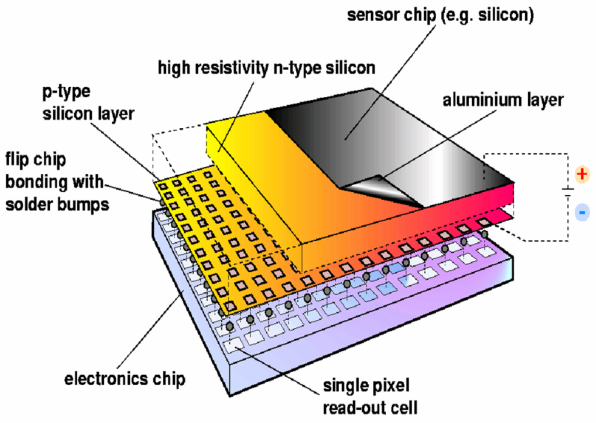
\includegraphics[width=0.35\textwidth]{minipix_silicon.pdf}
    \caption{MiniPIX silicon concept design}
    \label{fig:minipix_silicon}
\end{figure}
%
%figure name: minipix_silicon.pdf
%

%This was copied over to the "Experiment Design Section"
%For the SORA flights, the MiniPIX was coupled with a low cost open ARM based computer.  Both flights utilized a Raspberry Pi 3 to communicate and handle all operations with the MiniPIX.  This system allowed for remote operation and on-board analyzation of all data.  The SORA flights tested the feasibility of these low-cost systems to fly further space missions.  

%---Experiment Design ----- now called Methods ----- 05/05/2019 FIXED
\section{Methods}
\label{Methods}
% This should be fairly brief, the system is not particularly complex.
For the SORA flights, the MiniPIX was interfaced via USB with Raspberry Pi (RPI) single board computer as shown in Figure~\ref{fig:minipix_sch}. Data was collected on the MiniPIX and frame data was sent over serial to the RPI for analysis. During the 2017 flight, only the raw data was stored for post-flight analysis. For the 2018 flight, a custom piece of software was written to concurrently handle analyzing frame data, calculating absorbed dose and handling command and configuration requests from the HASP telemetry interface in addition to storing the raw data. The improvements in the 2018 flight allowed for a near real-time analysis of the radiation environment and the ability to configure the MiniPIX shutter rate and detector parameters via the HASP uplink interface. While being relatively cheap at a price point of 35\$ USD and consuming only \SI{1.2}{\watt} of electrical power, the RPI proved to be robust and operated without glitch for the duration of both flights.

\begin{figure}[H]
    \centering
    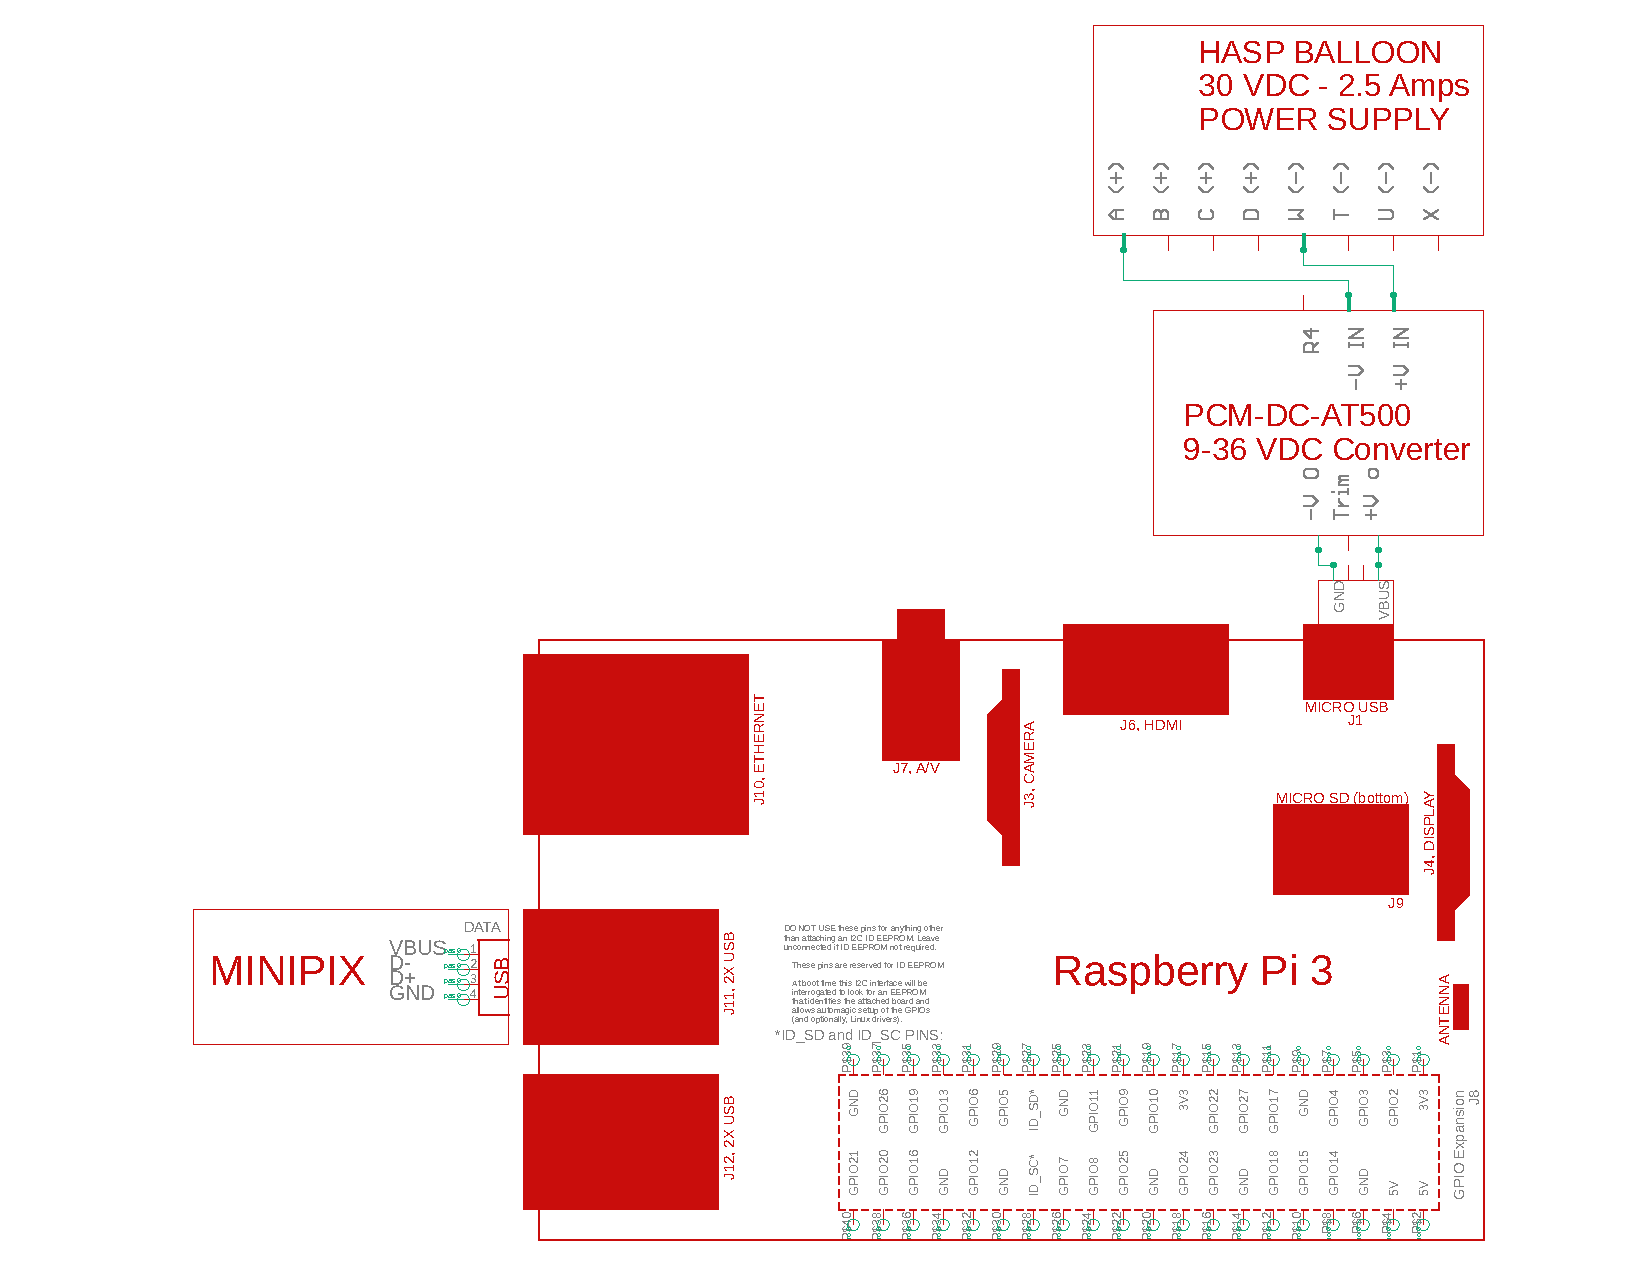
\includegraphics[width=.9\textwidth]{minipix_schematics.pdf}
    \caption{MiniPIX electrical schematic design.}
    \label{fig:minipix_sch}
\end{figure}


\subsection{Configuration and Calibration}
% Device parameters, threshold, bias voltage, shutter time etc.
The Timepix ASIC consists of 65,536 silicon p-n diodes, each containing its own individual processing circuit. The response of each pixel can never be identical, thus a calibration must be performed for each individual pixel. The appropriate calibration of the MiniPIX detector was applied at The University of Houston following a calibration procedure outlined by Jakubek \cite{mpjakubek}. The source calibration was applied using the 60 keV $^{241}$Am decay line, Sn Fluorescence and $^{55}$Fe gamma rays.
%REVIEW 1 from Renshaw: It would be good to show some result of this calibration, stating that the pixels were all calibrated to have response that is similar within some percentage of the average or even a histogram showing the spread of the calibration.

\subsection{System Design}
% RPI interface to MiniPIX, heatsink design etc.
Additive manufacturing was used to create a custom made case for the MiniPIX device.  The flight assembly is shown in Figure ~\ref{fig:minipix_case} with individual components as labeled.  In the early vacuum tests, it was found that the MiniPIX would require a passive cooling method to keep its temperature within operating limits.  At the same time, the ABS plastic enclosure acted as insulation, maintaining the MiniPIX temperature within the operating range.  The MiniPIX was mated to the heatsink via a bracket (not shown in the figure ~\ref{fig:minipix_case}) and with thermal adhesive.
\begin{figure}[H]
    \centering
    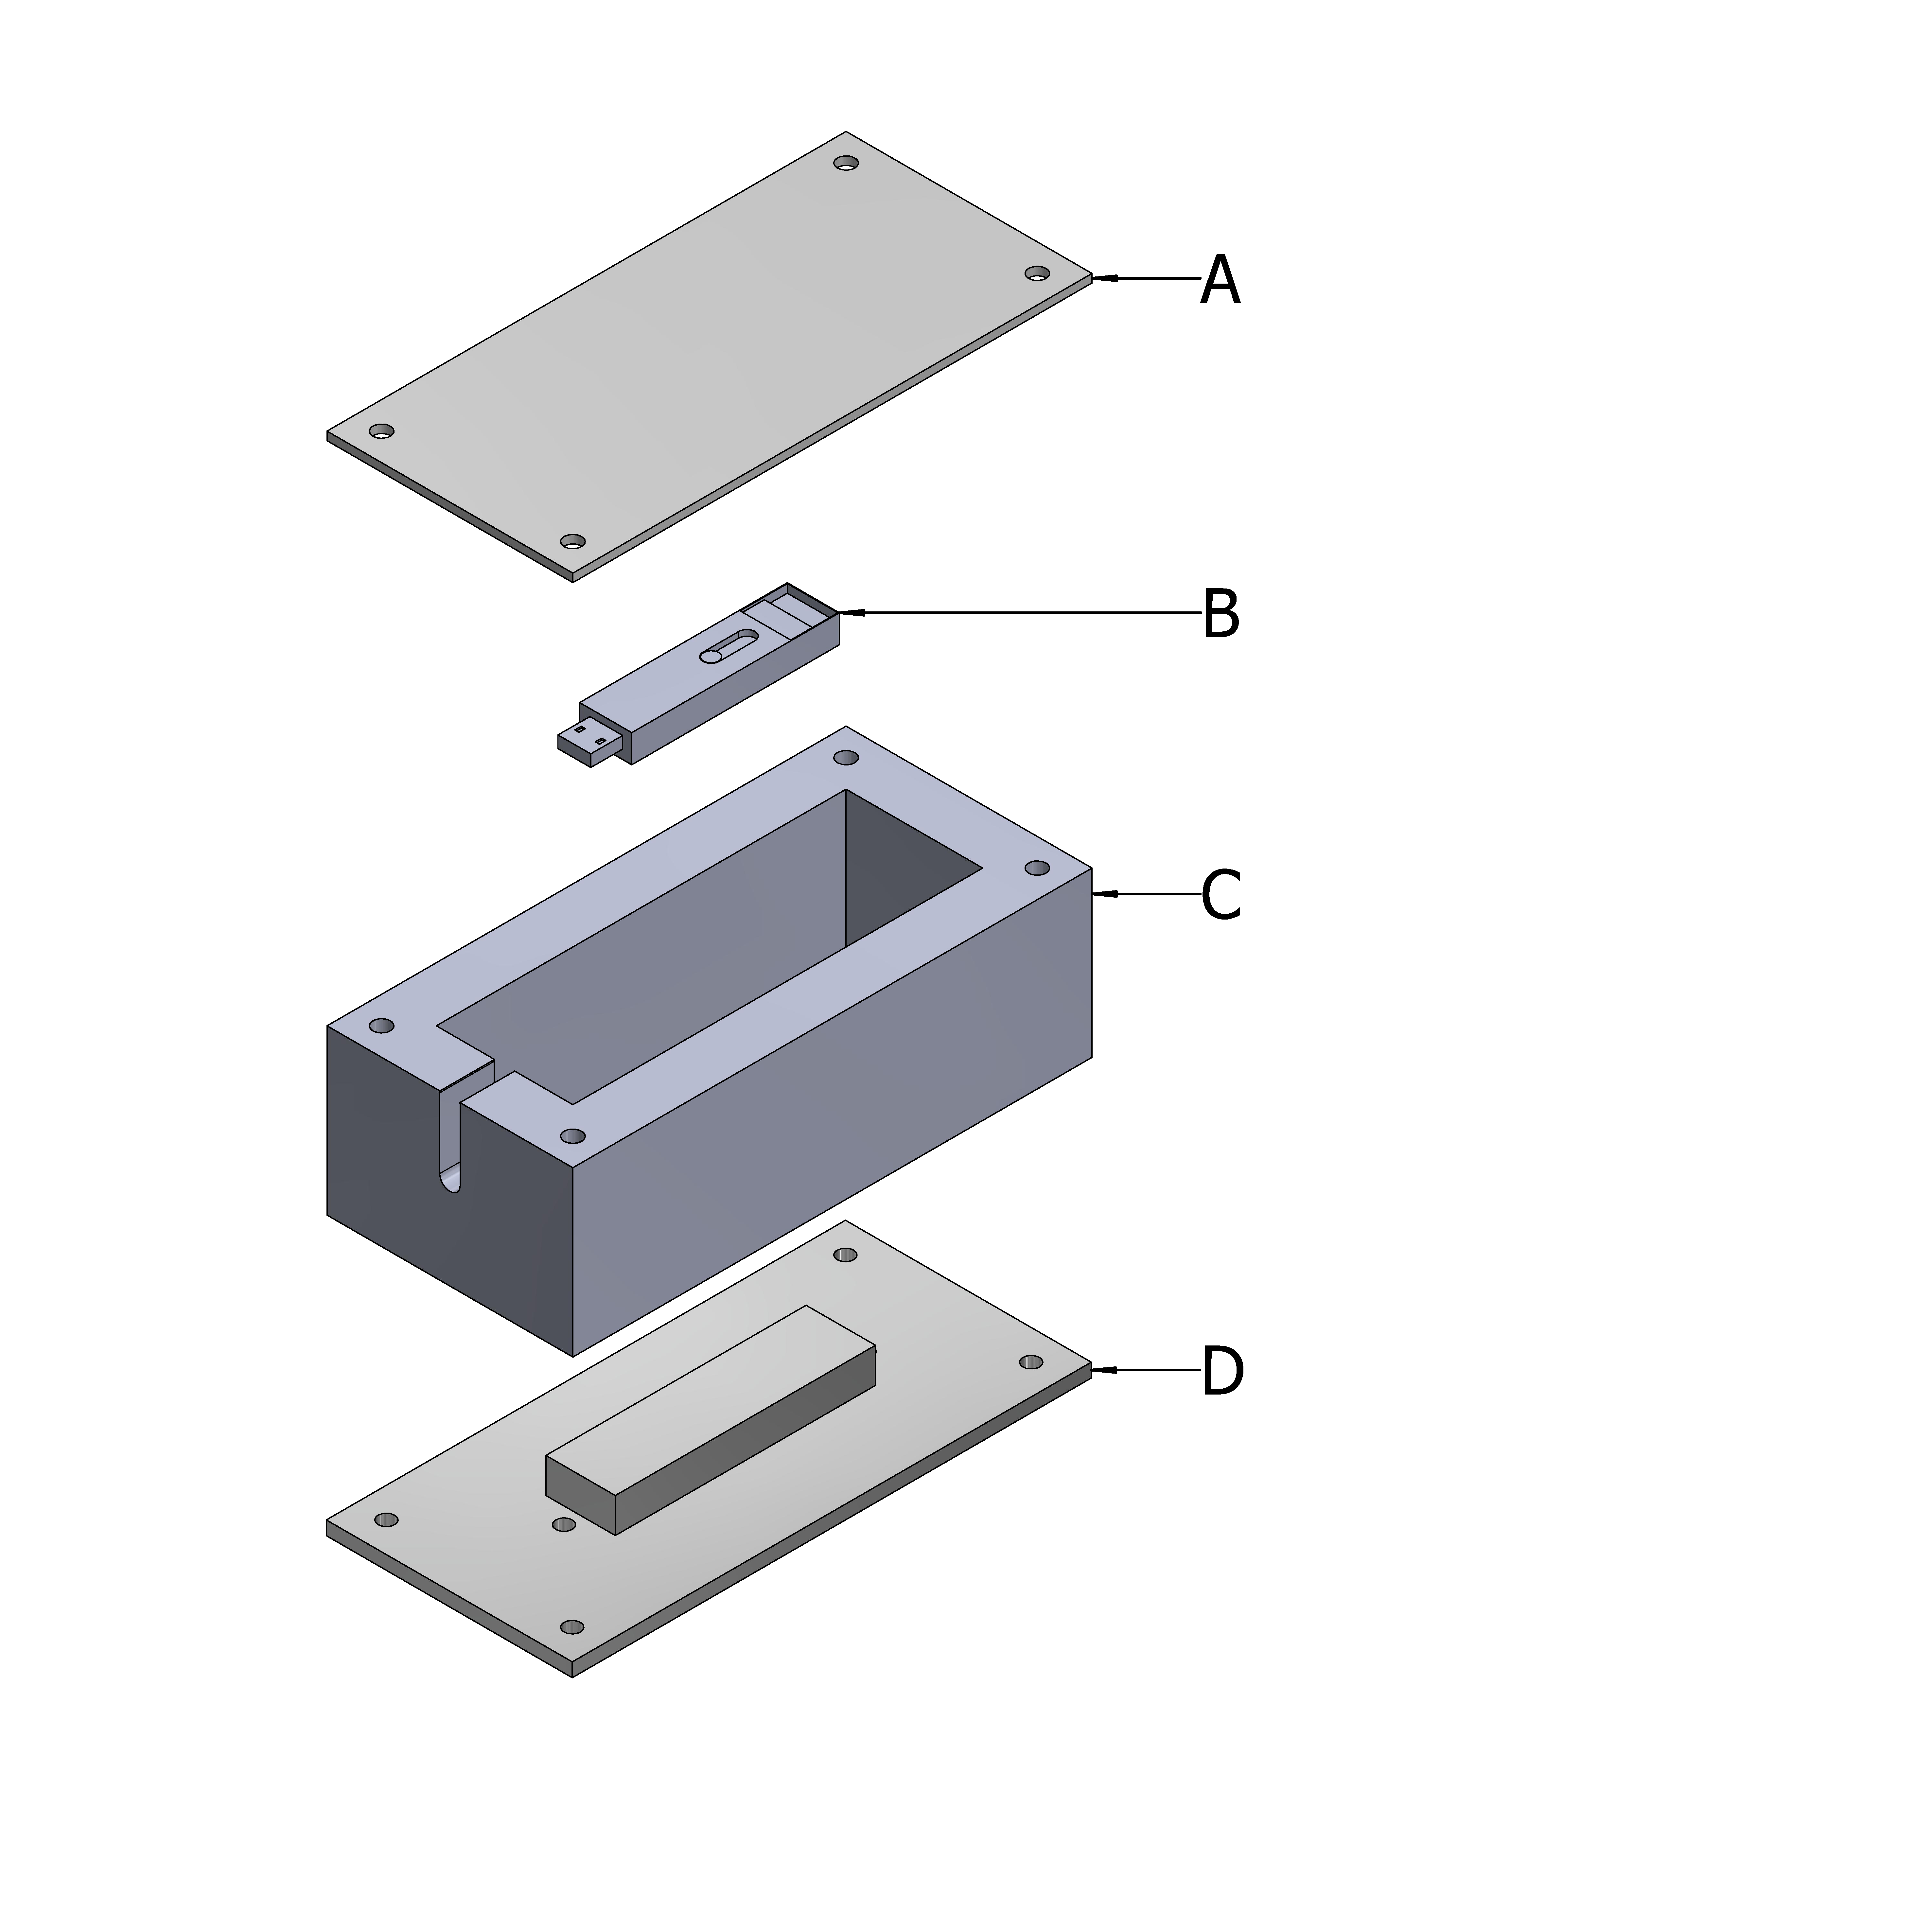
\includegraphics[width=0.45\textwidth]{Minipix_case_assembly.pdf} %from Sam - may need a better image from Steven but this will do for now, it includes all the main parts in a simple way.
%REVIEW 1 from Renshaw: It might be useful to make this a side-by-side figure, with the second figure being a CAD drawing or picture of the payload showing the placement of the RPI and the MiniPIX, along with the other components. 
    %%%Sam: upload new assembly picture
    \caption{MiniPIX~\cite{advacam} Case Assembly. A is the top case assembly, B is the MiniPIX USB device, C is the main case, and D is the heatsink assembly.}
    \label{fig:minipix_case}
\end{figure}
The MiniPIX case allowed for a USB cable to be routed through the enclosure to interface directly to the Raspberry Pi.  This allowed the MiniPIX device to be modular and placed in different configurations for the two flights.  The Raspberry Pi was placed in a separate location within each payload near the power supply.  Overall, each payload was modular and accessible.





%---Data Analysis ----- now called Results ---- 05/05/2019 FIXED
\section{Results}
\label{Results}
%\section{Data Analysis}
%\label{Data Analysis}

\subsection{Flight Data}
%Notes on how to take the results...
%What is being presented: Five plots total, the flight profile for each year, and cumulative dose for each flight.

\begin{figure}[H]
\centering
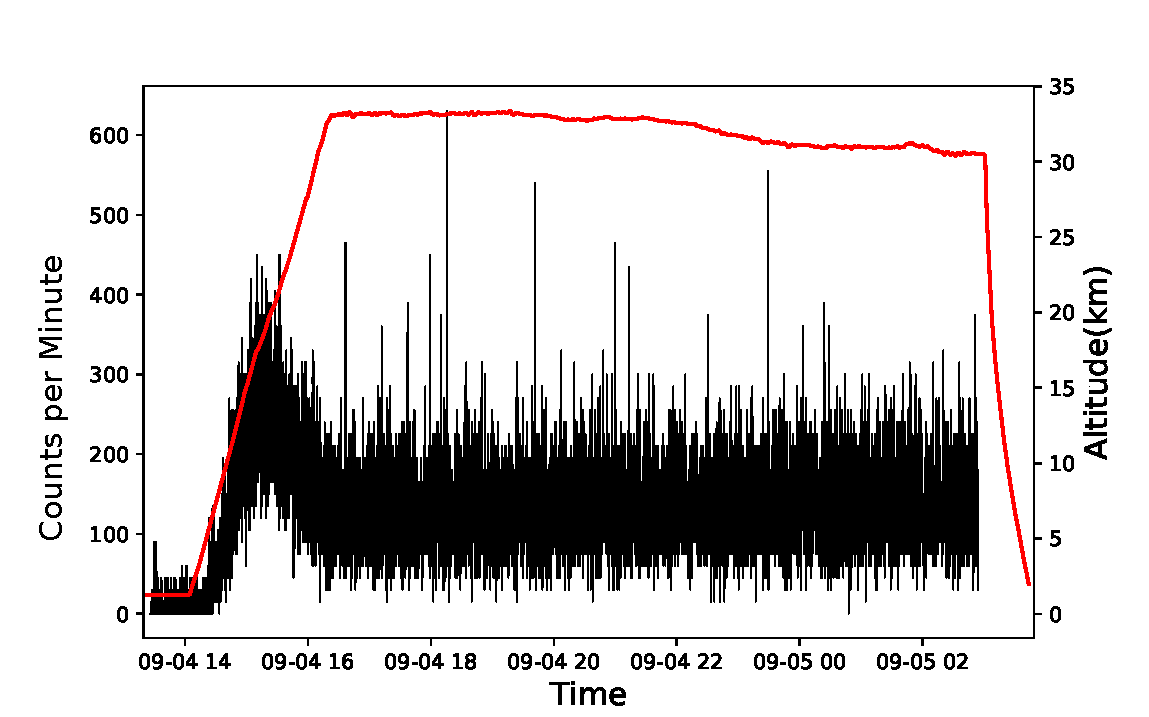
\includegraphics[scale=.75]{count_rate_altitude_2017_f.pdf} %REVIEW 1 from Renshaw: Enlarge this figure and remove the title from the top, titles are not shown in papers since the text and caption should tell you what they are.  Titles are only used in presentations and when sharing the figures around to other people without text or caption. Change the y-axis title to "Counts per Minute"
\caption{Count Rate and Altitude vs Time for 2017 flight. The red line represents the GPS altitude over time in \SI{}{\km}.  The black lines represent the counts per minute over time}
\label{fig:ratealttime_2017}
\end{figure}
%
%First:
%Present and characterize the first two plots - the data of the flight with counts vs altitude vs time.  Here we can talk about each flight and data shown.  Make sure to mention how the count rate changed as time and altitude changed.  We can talk about the flight time, the flight altitude variance, the coasting altitude, and how it all compares to the count rate.  We can be as descriptive as we can.
%mention the position of the pfotzer-regener maximum for both years.  Talk about discrepancies as the data shows.  Speculate in discussion later.
The MiniPIX was set to operate in Time over Threshold mode with a bias voltage of \SI{4}{\kilo\eV}.  Frames were collected at static 4 second intervals during the 2017 flight and between 1 and 4 second intervals for the 2018 flight.  The complete flight altitude profiles and count rates for the SORA  2017 and 2018 flights are shown in Figure~\ref{fig:ratealttime_2017} and Figure~\ref{fig:ratealttime_2018}, respectively.
%
\begin{figure}[H]
\centering
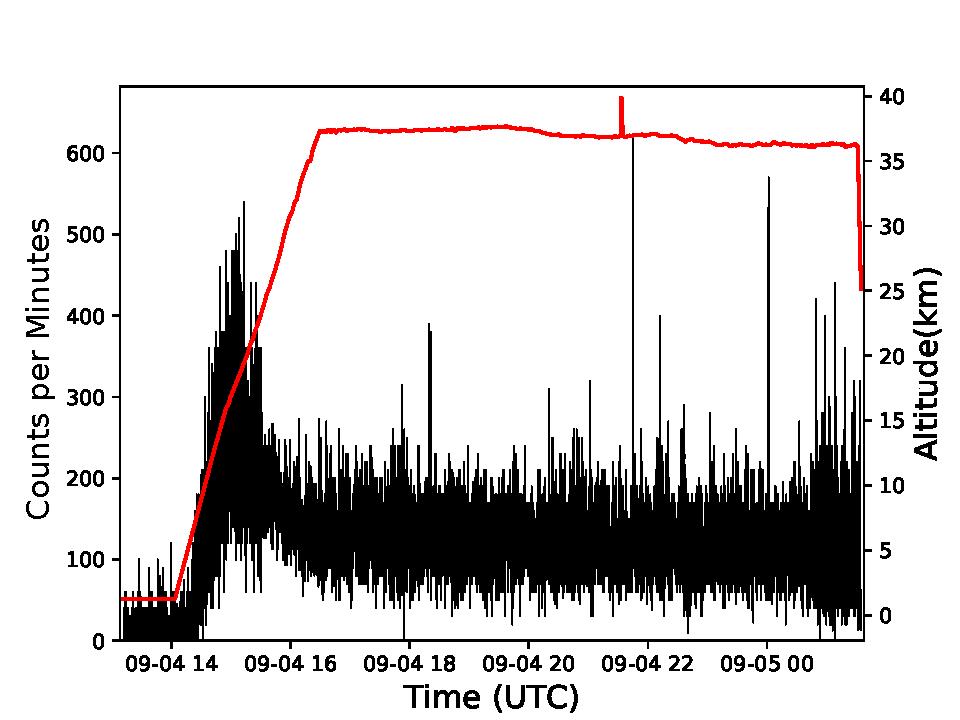
\includegraphics[scale=.80]{count_rate_altitude_2018_f.pdf}%REVIEW 1 from Renshaw: Enlarge this figure and remove the title from the top, titles are not shown in papers since the text and caption should tell you what they are.  Titles are only used in presentations and when sharing the figures around to other people without text or caption. Change the y-axis title to "Counts per Minute"
\caption{Count Rate and Altitude vs Time for 2018 flight. The red line represents the GPS altitude over time in \SI{}{\km}.  The black lines represent the counts per minute over time}
\label{fig:ratealttime_2018}
\end{figure}
%
As shown in Figure~\ref{fig:ratealttime_2017} and Figure~\ref{fig:ratealttime_2018}, both flights have very similar flight altitude profiles.  Both flights reached a float altitude after approximately \SI{2.5}{\hour}.  It is important to mention that the 2017 float altitude was approximately $\SI{31.5}{\kilo\meter}$.  While that for the 2018 flight was about $\SI{37.2}{\kilo\meter}$.  The rate of decent was slow and steady for both flights.  
%
As such, data was collected continuously throughout the whole flights. %%REVIEW 1 from Renshaw: Be careful about making this comment, based on the two figures, we see the altitude go almost to 0 for 2017, but the data stops before this, while for 2018 the plot cuts off the decent and so it is not clear where the data taking stopped.  I think you should rephrase this to say that data was taken during the entire ascent and float periods of both flights and don't mention anything about the decent since it happened much quicker than the ascent and also in a much less controlled manner since the payload was spinning out of control at that point.
%

\begin{figure}[H]%%%REVIEW 1 from Renshaw: You may want to reverse the order of these two plots, since I believe the count rate is the more fundamental quantity and dose rate is something that extends the count rate based on the energy that is deposited.  Also, Change y-axis title to Counts per Minute, it would also be good to enlarge these figures as much as possible without making them take up an entire page.  Remove the titles from each of the plots. Remove this part of the caption, there is no need or it since this information is given in the real caption.
\centering
\begin{subfigure}{.5\textwidth}
  \centering
  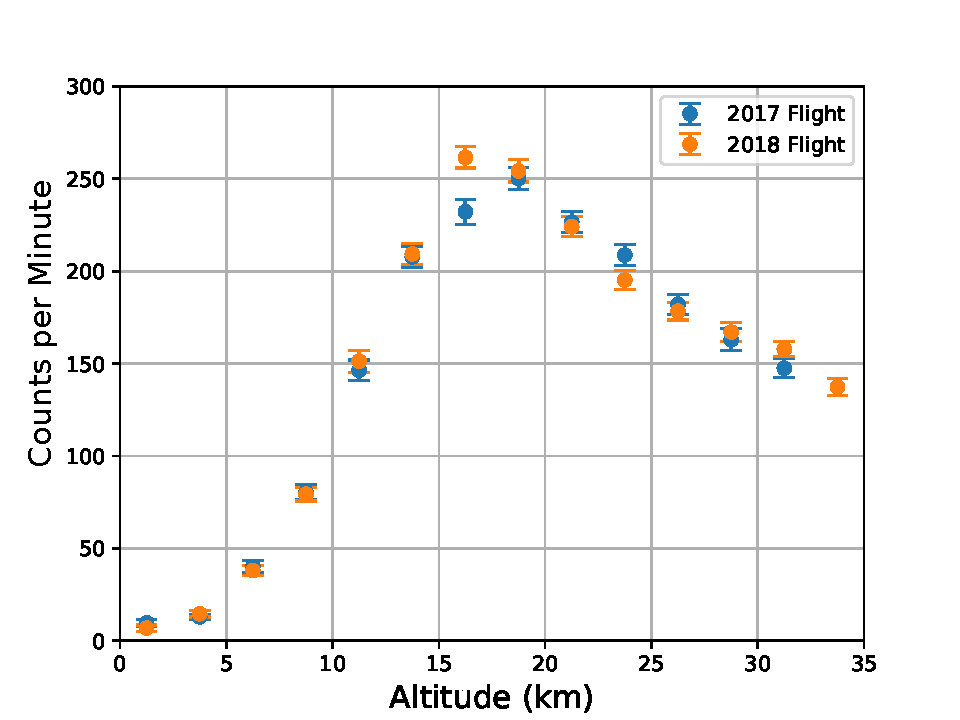
\includegraphics[scale=.45]{cva_stderr_f.pdf}
  \caption{}
  \label{fig:sub2}
\end{subfigure}%
\begin{subfigure}{.5\textwidth}
  \centering
  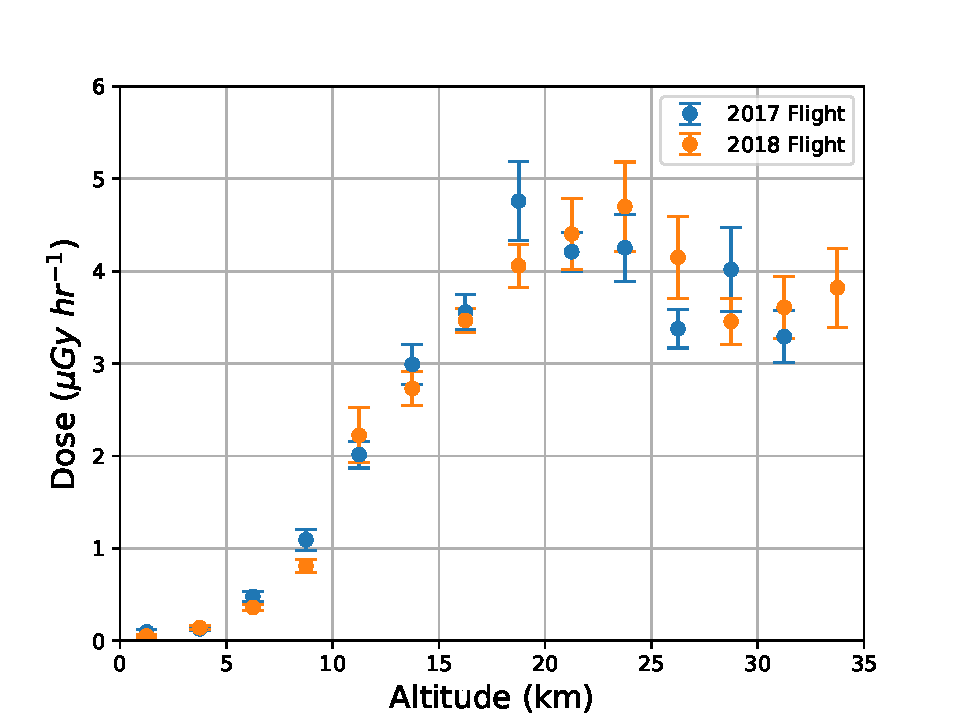
\includegraphics[scale=.45]{dva_stderr_f.pdf}
  \caption{}
  \label{fig:sub1}
\end{subfigure}%
\caption{Figure ~\ref{fig:sub2} shows the detector counts per minute as a function of GPS altitude. Figure ~\ref{fig:sub1} shows the absorbed dose rate in silicon as a function of GPS altitude.  Samples were averaged over \SI{2.5}{\kilo\meter} bins and error bars for both plots represent the standard error of the mean plotted at the $1\sigma$ level.}
\label{fig:dose-count-subplots}
\end{figure}

%% left old here just in case we need to revert
%\centering
%\begin{subfigure}{.5\textwidth}
%  \centering
%  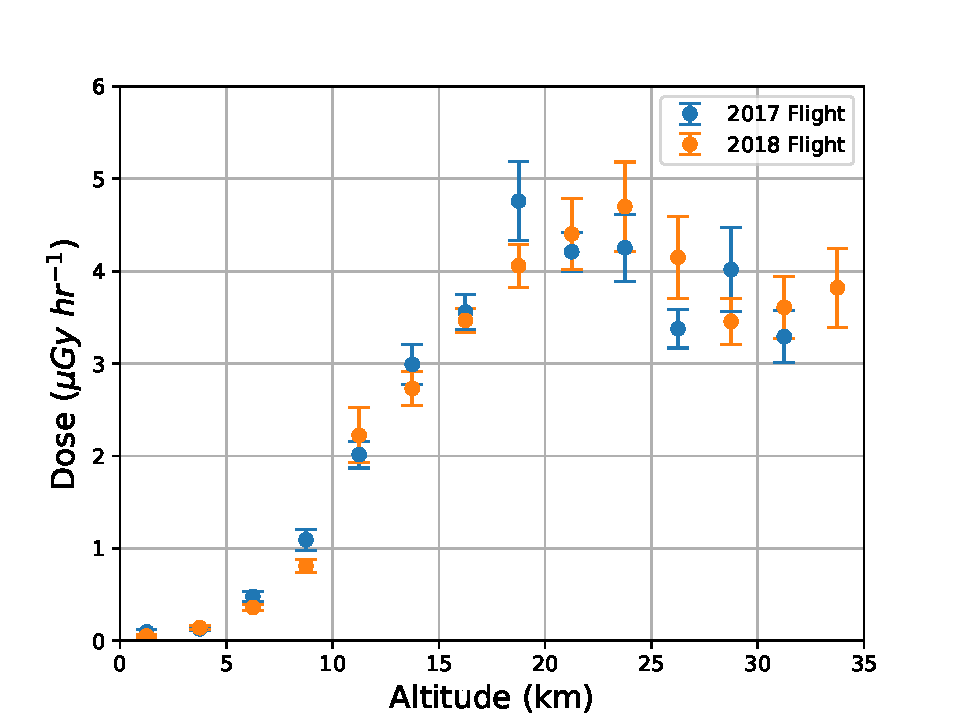
\includegraphics[scale=.45]{dva_stderr_f.pdf}
%  \caption{}
%  \label{fig:sub1}
%\end{subfigure}%
%\begin{subfigure}{.5\textwidth}
%  \centering
%  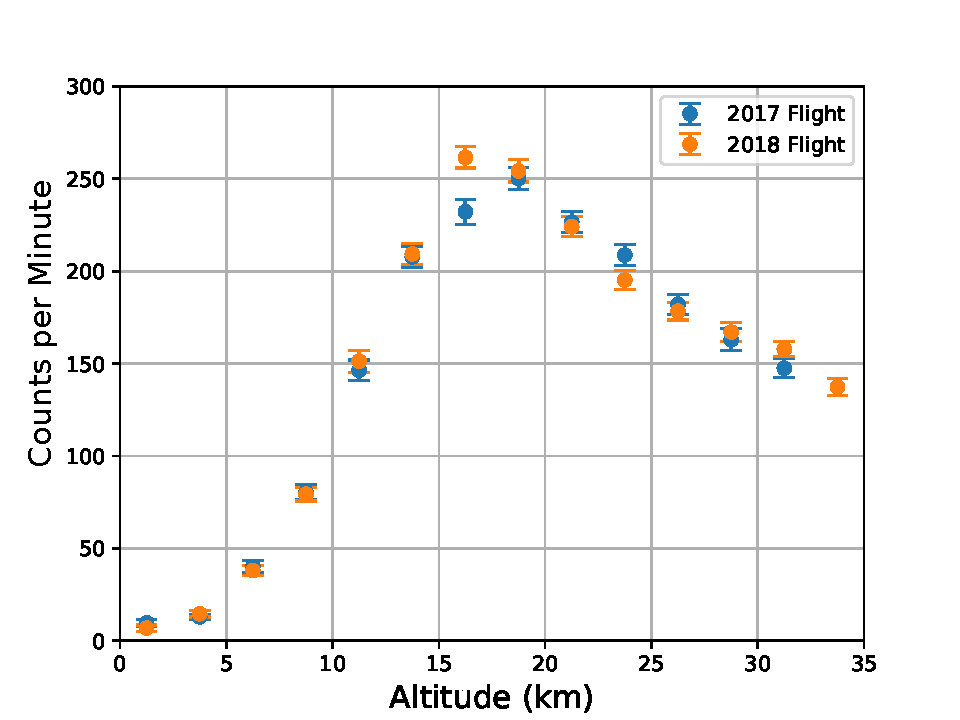
\includegraphics[scale=.45]{cva_stderr_f.pdf}
%  \caption{}
%  \label{fig:sub2}
%\end{subfigure}
%\caption{Figure ~\ref{fig:sub1} shows the absorbed dose rate in silicon as a function of barometric altitude.  Figure ~\ref{fig:sub2} shows the detector counts per minute as a function of barometric altitude. Samples were averaged over \SI{2.5}{\kilo\meter} bins and error bars for both plots represent the standard error of the mean plotted at the $1\sigma$ level.}
%\label{fig:dose-count-subplots}
%\end{figure}
%Next, go into the absorbed rate vs altitude plot.  Mention how the LET varies for materials such as silicon and muscle.  Go into the pfotzer-regener maximum again, compare.  Compare this to the accompanying figure, Detector Hits vs Altitude.  There is a slight discrepancy in the flights, this may be useful to mention.  All error bars are 1 sigma standard deviation.
Shown in Figure~\ref{fig:sub1} and Figure~\ref{fig:sub2} are the dose rate in silicon and the detector count rate plotted as a function of GPS altitude. For the sake of clarity samples were averaged over \SI{2.5}{\kilo\meter} bins and plotted with error bars representing the standard error of the mean at the $1\sigma$ level. Dose rates for both flights appear to be in relatively good agreement up until approximately \SI{16}{\kilo\meter}. After which, the 2017 flight appears to reach a peak dose rate of \SI{4.8}{\micro\gray\per\hour} at approximately \SI{18}{\kilo\meter} while the 2017 flight reaches a peak of \SI{4.8}{\micro\gray\per\hour} at a higher altitude of \SI{24}{\kilo\meter}. 
%
However, the large error bars indicate that it is somewhat unclear as to where the peak dose rate occurs for both flights. %%REVIEW 1 from Renshaw: I would suggest to try and make a fit to the two data series with some function that is taken from a reference which provides the expected rate, this would be a good way to then state what the maximum is and where it is located, with the fit also producing the uncertainty of the location of the max.
%
The dose rates for both flights seem to be in much better agreement than the count rates and show only a small discrepancy between \SI{15}{\kilo\meter} and \SI{17.5}{\kilo\meter} at which the 2018 flight experienced a count rate approximately 30 counts per minute higher than that of the 2017 flight. %%REVIEW 1 from Renshaw:Do we have any idea why this discrepancy is here?  If so it would be good to make a statement about it here. 
%
With both flights reaching altitudes beyond $\SI{25.0}{\kilo\meter}$, the Pfotzer-Regener maximum was clearly observed.  
%
In 2017, the Pfotzer-Regener maximum peaked at approximately  $\SI{18}{\kilo\meter}$.  Similarly, the 2018 mission recorded Pfotzer-Regener maximum peaking around $\SI{20}{\kilo\meter}$. %%REVIEW 1 from Renshaw: Would be good to give the current accepted altitude of the P-R maximum and the reference which states this, then we can directly compare this measurement to that which is accepted 
%
After the observed peaks in count rate, the count rate tapered off inversely with rising altitude.  These count rates then remained constant for the remainder of the flights. %REVIEW 1 from Renshaw: until the float altitude was reached, at which point the count rate remained a constant value, within the uncertainty of the measurement. 

%
%The Pfotzer-Regener maximum is clearly visible between \SI{15}{\kilo\meter} and \SI{20}{\kilo\meter} for both years in both absorbed dose and count rate. 
%
%Variation year over year in measurements of absorbed dose and counts is to be expected and is likely a reflection of the ongoing solar minimum. (need to expand on this a little...)
%
%Another area for the discussion - great area to talk about the discrepancies.  Here we only talk about data and thats it.
%
%Similarly, Figure~\ref{fig:sub2} again confirms the Pfotzer maximum reached for both years.
%For discussion: Here the error is more consistent and Pfotzer maximum is reached at the expected altitudes.

\begin{figure}[H]
\centering
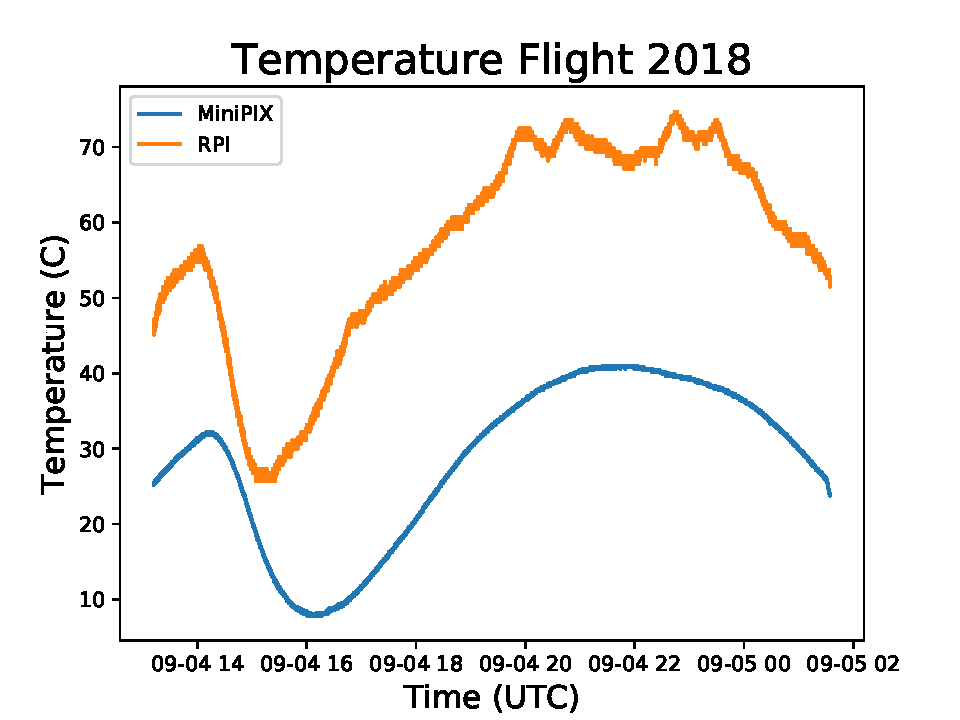
\includegraphics[width=\textwidth]{temps_flight_2018.pdf} %REVIEW 1 from Renshaw: Move this figure and the text associated with it to before the figures and text about the dose rate and count rate. Remove the title from this plot.  Add the degrees symbol to the units for y-axis before the 'C'.
\caption{2018 recorded temperatures of the MiniPIX and Raspberry Pi Flight computer.}
\label{fig:temps_2018}
\end{figure}
%
The MiniPIX and RPI both operated well throughout both flights.  The 2018 flight was better equipped to record system health and operation status.  A key status indicator of system health was the system temperature.  These temperatures recorded are shown in Figure~\ref{fig:temps_2018}.  The MiniPIX temperature stayed within expected ranges and never exceeded $\SI{40}{\degreeCelsius}$.  Likewise, the RPI stayed with operational temperatures.
%FOR Discussion - compare to BEXUS flights and RADX flight as well, and mention how the maximum is similar/different.  Here the maximum in the Hands et al RaD-X mission found the Pfotzer maximum around 60,000 ft (~18 km).  
%
%
%
\begin{figure}[H]
\centering
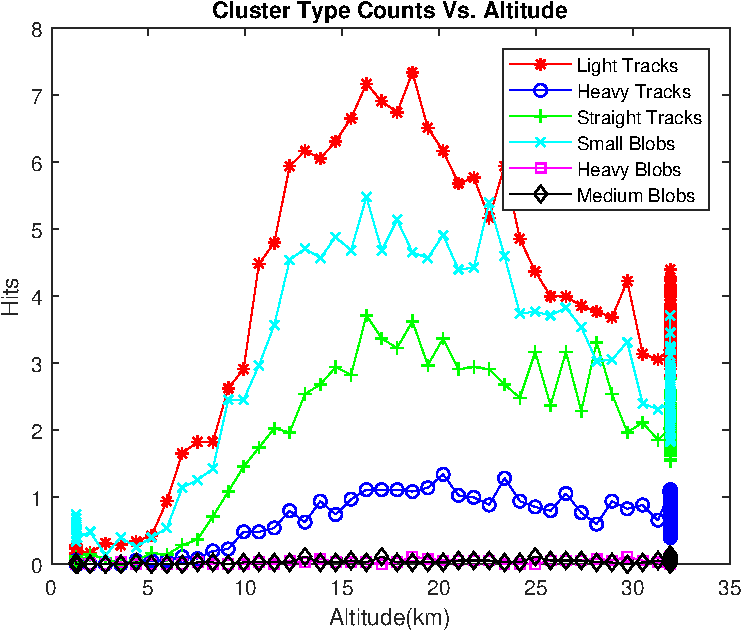
\includegraphics[width=\textwidth]{ctva-cropped.pdf} %% REVEIW 1 from Renshaw: Remove the title from plot.  Make the legend smaller or move it so it does not overlap with the data series.  Put a space between 'Altitude' and '(km)'.  Change y-axis title to 'Number of Hits'. The number of data points at float altitude is confusing and makes the plots hard to read, I would suggest to take an average of these for each data series and then show a single data point for each of them at the float altitude, make sure to take the error bars into account properly when doing the average such that the final error bar represents the spread in the points here
\caption{Distribution of cluster type counts versus altitude for the duration of the 2018 flight.}
\label{fig:cluster2018}
\end{figure}
%Finally, the last figure Cluster Type Counts vs Altitude.  This is useful due to the MiniPIX being able to analyze individual track lengths.  From here, these tracks can be characterized into different and individual categories.  This is useful for LET calculations and overall more precise for dosage calculations.  It may also help with particle identification.
The distribution of cluster types as they vary with altitude is shown in Figure~\ref{fig:cluster2018}.  %%REVIEW 1 from Renshaw: This part needs to be greatly expanded to include the description of what each of the event cluster types are, and then also what type of particles could potentially result in each of the cluster types.  It would also be good to have a figure which shows 6 frames from the MiniPIX, each one giving an example of each of the cluster types so that the reader can see what they actually look like compared to each other.  I imagine that this figure could be laid out in a 2x3 matrix and inserted as a single figure into the paper.
%
%%Sam Changes in response to above review 07/26/12019
%
%\begin{figure}[H]
%\centering
%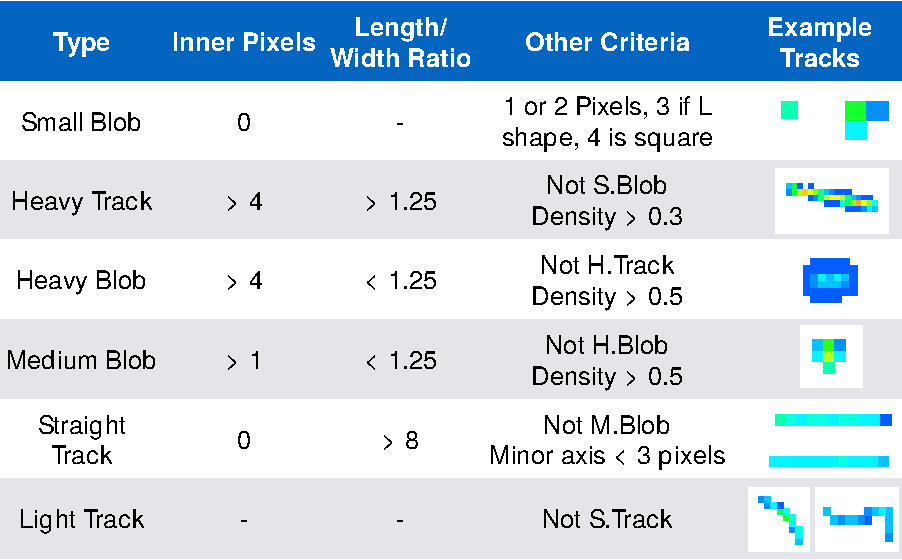
\includegraphics[width=\textwidth]{stuartgraphic.pdf}
%\caption{Cluster types\cite{stuartalgo}} %%%NEED CITATION
%\label{fig:stuartfigure}
%\end{figure}
%
%%End Sam Changes 07/26/2019
%
\begin{figure}[H]
\centering
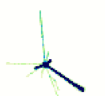
\includegraphics[width=\textwidth]{tracks.pdf} %No need to give the frame number here, can be removed from the figure and inserted into the caption if you want. It might be good to move this figure and the text for it to before the previous figure and its text, since it would be good to show an example frame and describe that the energy is measured from the track length.  Then show the figure with the different types of clusters, and then the figure with the rate of each of them.  This would be a more logical order in terms of building the understanding for the reader. It would be good to explain this figure better in the text.  So what are each of the numbers in the frame, and why does the large cluster/track look the way it does?
\caption{Single MiniPIX frame collected at float on the 2017 flight.}
\label{fig:frame1}
\end{figure}
Figure~\ref{fig:frame1} shows one of many particle tracks recorded during the 2017 flight, while both flights recorded many frames similar to this.  The track lengths of ionizing particles can be calculated and used to directly measure the linear energy transfer of various primary and secondary particles.




%---Discussion
%Report results first, including figures, particle count, dose, altitude, and temperatures.

\section{Discussion}

\label{Discussion}

%Introduce the basic system again and how it was briefly setup.

%Discuss dose and particle count measurements as they relate to classical theory

%Talk about the success of the overall PAYLOAD briefly.

% Talk about cumulative dose somewhere.

A primary goal of the SORA flights was to successfully utilize the MiniPIX device in dosimetric applications.

The figures presented in Section \ref{Results} clearly demonstrate this success as the results from the two missions are validated by comparison to previous stratospheric balloon flights.

The BEXUS \cite{bexus} balloon flights have shown that Medipix sensors are able to perform in the stratosphere.

NASA's RaD-X missions \cite{rad-x} provided unprecedented results to which SORA's data can be compared.



\subsection{System Performance}

% Here its just specific discussion about the system performance.

% Talk about success of overall SYSTEM.  Include TEMP data about the flight and hardware of the system.  Mention altitude, humidity, and any atmospheric conditions available for both flights.

Due to the lack of heat convection in the stratosphere, a pressing concern regarding the functionality of the MiniPIX was the temperature of the device at float altitude. 

The device is guaranteed to operate within the manufacturer's limits of \SIrange{0}{70}{\celsius}.

With the use of a relatively compact heatsink, the temperature of the device remaned within \SIrange{10}{40}{\celsius}.

The success of the heatsink suggests that less material could be utilized, consequently reducing the overall size of the apparatus.



\subsection{Space Weather}

% Relevancy of space weather to commercial airlines.

% Astronauts' time in space is decreasing.

% Mention the issues with modeling aviation radiation exposure with simulations as opposed to real data. I found a paper from one of the RaD-X authors that details this point: https://agupubs.onlinelibrary.wiley.com/doi/10.1002/2016SW001399



\subsection{Success of SORA Relative to Others}

% Detail the results which match the NASA article

The success of the application of the MiniPIX as a dosimeter is clearly seen with direct comparison to the RaD-X missions. Figure \ref{fig:sub1}

The absorbed dose measured by SORA is slightly higher that that measured by the RAD-X.

This can be explained by the difference of the year of each flight and the relationship between the solar cycle and GCR flux.

The solar cycle is inversely related to GCR flux \cite{hathaway}, i.e. when the sun is at solar minimum the GCR flux is at a maximum.

The RaD-X mission was in 2015 during the decline of the current solar cycle, solar cycle \num{24}. 

Solar cycle 24 hit its solar minimum in March 2018, only a few months prior to the second SORA flight in September 2018.





% Explain how we expanded upon their work, but that there is still much more than can be done.

% Mention the need for a low-cost dosimeter and how our configuration is reaching that goal. The only setback in the high-cost of the commercially unavailable MiniPIX.

% Mars environment

%---Conclusion
\section{Conclusion}
\label{Conclusion}
% Report Findings, report what the overall goal of the project and if the goals were met in the end.

Overall, the device performed adequately and is potentially suitable for future applications in other areas...


% Discuss briefly (IN ONE OR TWO SENTENCES) future applications of the MiniPIX for compact, cheap and accurate(?) dosimeters on commercial airline flights
%THIS FITS BETTER SOMEWHERE ELSE; INTRODUCTION, BACKGROUND AND DISCUSSION.
%The authors of this paper have made arrangements to collaborate with Dr. Lawrence Pinsky and Dr. Stuart George of the University of Houston to develop a portable, TimePIX-based device capable of detecting thermal neutrons. The motivation behind this project is to investigate the production rates of and passenger exposure to thermal neutrons during commercial air flights by building off of the previous work done by groups such as B.J. Lewis et al. \cite{aircrewexposure} and C. Granga and S. Pospisil \cite{timepixdosimetry}.


%---Acknowledgements
%Acknowledgements
%Collate acknowledgements in a separate section at the end of the article before the references and do not, therefore, include them on the title page, as a footnote to the title or otherwise. List here those individuals who provided help during the research (e.g., providing help during the assembly process, language help, writing assistance or proof reading the article, etc.).

\section{Acknowledgements}
\label{Acknowledgements}
Dr. T. Gregory Guzik @ LSU % https://www.lsu.edu/physics/people/faculty/guzik.php
Louisiana Space Group for supporting HASP flights

NASA Balloon Program Office for supporting HASP flights

NASA Columbia Scientific Balloon Facility for supporting HASP flights

University of Houston Physics Department

University of Houston Biology and Microbiology Department

University of Houston STEM Center

Dr. Jacobs at the UH STEM Center

Randy Clark at the UH Science Center Machine Shop - Lab Machinist




%---Funding Sources
\section{Funding Sources}
\label{funding}
This work was supported by the University of Houston STEM Center.


%---Appendix
%% The Appendices part is started with the command \appendix;
%% appendix sections are then done as normal sections
%% \appendix

%% \section{}
%% \label{}


%---Bibliography
%% References
%%
%% Following citation commands can be used in the body text:
%% Usage of \cite is as follows:
%%   \cite{key}          ==>>  [#]
%%   \cite[chap. 2]{key} ==>>  [#, chap. 2]
%%   \citet{key}         ==>>  Author [#]

%% References with bibTeX database:
%%%%%%%%
%%%%%%%%\bibliographystyle{model1-num-names}
%%%%%%%%\bibliography{sample.bib}

%% Authors are advised to submit their bibtex database files. They are
%% requested to list a bibtex style file in the manuscript if they do
%% not want to use model1-num-names.bst.

%% References without bibTeX database:

\begin{thebibliography}{00}

%% \bibitem must have the following form:
%%   \bibitem{key}...
%%

%\bibitem{SORA}S.A. Garcia Morelos, F.Brooks, S.Oliver, A.Walker, K.D. Portillo, R.B. Masek, D.Mroczek, D.Pena, J.Juarez, A.Cruz, D. Henandez, S.George, D. Pattison, A.L.Renshaw. \textit{Scientific Report for the UH Team.} SORA 2017 Mission Webpage. \textit{http://laspace.lsu.edu/hasp/groups/Payload.php?py=2017&pn=10}.

\bibitem{minipix}MiniPIX - Miniaturized Portable USB Photon Counting Camera. (n.d.). Retrieved February 02, 2017, from \textit{http://advacam.com/camera/minipix}.

%\bibitem{LSU}
%  Christner, B., Alleman, M., Bryan, N., Burke, S., Guzik, T.G., Granger, D., King, G. (2013) \textit{LSU HASP2013 PDF. Baton Rouge: Louisiana Space Consortium}.
%
%%\bibitem{SolidWorks}
%%  SolidWorks 3D CAD software \url{http://www.solidworks.com/}.
%
%\bibitem{Extremophiles}
%  Extremophiles \href{http://www.nytimes.com/2013/02/07/science/living-bacteria-found-deep-under-antarctic-ice-scientists-say.html}{http://www.nytimes.com/2013/02/07/science/living-bacteria-found-deep-\\under-antarctic-ice-scientists-say.html}.
%
%\bibitem{canales}
% Canales D. C. and Ehteshami A., \textit{An attempt to sample atmospheric bacteria}, Houston, TX, 2015, January 11.
%
%\bibitem{bexus}
%Urbar, J., Scheirich, J., Jakubek, J., 2011. Medipix/Timepix cosmic ray tracking on BEXUS stratospheric balloonflights. Nucl. Instrum. Methods A 633, S206-209.
%	
%%\bibitem{uv_irradiance}
%%  Calculating the UV Index. (2016, October 14). Retrieved June 03, 2017, from \url{https://www.epa.gov/sunsafety/calculating-uv-index-0}.
%
%%\bibitem{cleanbox}
%% Clean box material \url{https://www.mcmaster.com/\#uhmw-polyethylene/=1aijn1p}.
%
%\bibitem{valve}
% Valve data sheet \url{http://www.generant.com/Literature/Series\%20VRV\%20Product\%20Literature.pdf}.
%
%\bibitem{advacam}
%  ADVACAM at \url{advacam.com}.
%
%\bibitem{medipix}
%  Medipix collaboration at \url{https://medipix.web.cern.ch/}.
%  
%\bibitem{stuartthesis} 22
%  George, S., \textit{Dosimetric Applications of Hybrid Pixel Detectors}, University of Wollongong, Australia, 2015.
%
%%\bibitem{mpdatasheet}
%%  ADVACAM, \textit{MINIPIX Version 1.0 Datasheet}, Retrieved from \url{http://www.widepix.cz/files/datasheets/MiniPIX\%20v1.0\%20Datasheet.pdf}.
%
%%\bibitem{mpjakubek}
%%  Jan Jakubek, \textit{Precise energy calibration of pixel detector working in time-over-threshold mode} Institute of Experimental and Applied Physics, Czech Technical University in Prague, Czech Republic, 2011.
%  
%
%    
%
%
%%\bibitem{magnetictool}
%%  United States National Oceanic and Atmospheric Administration, \textit{Magnetic Field Calculators} [Data sets], Retrieved from \url{https://www.ngdc.noaa.gov/geomag-web/#igrfwmm}.
%
%%\bibitem{gorman}
%%	Gorman, J. (2013, February 06). \textit{Scientists Find Life in the Cold and Dark Under Antarctic Ice.} Retrieved September 15, 2016, from Scientists Find Life in the Cold and Dark Under Antarctic Ice.
%	
% 
% 
%%\bibitem{pumpsource}
%%  \url{http://www.knfusa.com/?type=5600&amp;file=2079}.
%
%
%%\bibitem{Horneck}
%%  Horneck, G. 1993. The Biostack concept and its application in space and at accelerators: studies in Bacillus subtilis spores, p. 99-115. In C. E. Swenberg, G. Horneck, and E. G. Stassinopoulos (ed.), \textit{Biological effects and physics of solar and galactic cosmic radiation}[PDF], part A. Plenum Press, New York, NY. accessed 10/24/16  
%
%%\bibitem{Horneck} 
%%  Horneck, G. 2007. \textit{Space radiation biology}[PDF], p. 243-273. In E. Brinckmann (ed.), Biology in space and life on Earth. Wiley-VCH, Weinheim, Germany. Accessed 10/26/16
%
%%\bibitem{Horneck}
%%  Horneck, G., C. Baumstark-Khan, and G. Reitz. 2002. \textit{ Space microbiology: effects of ionizing radiation on microorganisms in space}[PDF], p. 2988-2996. In G. Bitton (ed.), The encyclopedia of environmental microbiology. John Wiley \& Sons, New York, NY. Accessed 10/30/16
%
%%\bibitem{Horneck}
%%  Horneck, G., C. Baumstark-Khan, and R. Facius. 2006. \textit{Radiation biology}[PDF], p. 292-335. In G. Cl?ment and K. Slenzka (ed.), Fundamentals of space biology. Kluwer Academic Publishers/Springer, Dordrecht, The Netherlands. accessed 11/4/16
%
%%\bibitem{Kiefer}
%%Kiefer, J., K. Schenk-Meuser, and M. Kost. 1996. \textit{Radiation biology}[PDF], p. 300-367. In D. Moore, P. Bie, and H. Oser (ed.), Biological and medical research in space. Springer, Berlin, Germany. accessed 11/9/16
% 
%	
%
%\bibitem{SamURD}
%	Alfonso Garcia Morelos, S. (2016, October 13).
%	\textit{A Novel Microbe Trap.}
%	Presentation at UH Undergraduate Research Day. \url{http://www.uh.edu/honors/undergraduate-research/}
%	
%	
%%\bibitem{StevenURD}
%
%%\bibitem{FreEttaWomensConference}
%
%%\bibitem{StevenSchoolPres}
%
%%\bibitem{StevenURD}
%%  Oliver, S. J. (2017, October 12). 
%%  \textit{Stratospheric Organism and Radiation Analyzer}
%%  Presentation at UH Undergraduate Research Day. Retrieved October 12, 2017, from \url{http://www.uh.edu/honors/undergraduate-research/events/urday2017/}
%
%%\bibitem{StevenSchoolPres}
%%  Oliver, S. J. (2017, November 4). 
%%  \textit{STEM Life at UH}
%%  Presentation at UH Gathering of the Eagles STEM Symposium. \url{https://www.uh.edu/news-events/stories/2016/November/110416EaglesSTEM.php}
%
%%\bibitem{Fre}
%%  Brooks, F. (2017, January 14).
%%  \textit{Stratospheric Organism and Radiation Analyzer}
%%  Presentation at Rice University, APS Conferences for Undergraduate Women in Physics (CUiP). \url{http://www.google.com/url?q=http%3A%2F%2Fwww.aps.org%2Fprograms%2Fwomen%2Fworkshops%2Fcuwip.cfm&sa=D&sntz=1&usg=AFQjCNE5pImV-SVrb87CvgAa9RSfeCrYXg}  
%  
%%\bibitem{SamAPS}
%%	Alfonso Garcia Morelos, S. (2017, October 20).
%%	\textit{Stratospheric Organism and Radiation Analyzer}
%%	Retrieved October 20, 2017, from \textit{Bulletin of the American Physical Society}. \url{https://meetings.aps.org/Meeting/TSF17/Session/E5.3}
%	
%  
%%  \bibitem{MIT}
%%	MIT-Lemelson Award 2018.
%%	\url{https://lemelson.mit.edu/}

\end{thebibliography}




\end{document}

%%
%% End of file `elsarticle-template-1-num.tex'.
              
\grid
\grid
